\section{Method of the characteristics}

\manuelComment{based on this video: https://www.youtube.com/watch?v=LpHqrlrU5pM}

The method of the characteristics is a powerful method to solve PDE. This method enable us to solve a wide range of problems including:
\begin{enumerate}
  \item Linear:
  \begin{equation}
  a(x, y) \frac{\partial u}{\partial x}
  + b(x, y) \frac{\partial u}{\partial y}
  + c(x, y) u
  = f(x, y)
  \end{equation}
  \item Semi-linear:
  \begin{equation}
  a(x, y) \frac{\partial u}{\partial x}
  + b(x, y) \frac{\partial u}{\partial y}
  + c(x, y) u
  = f(x, y, u)
  \end{equation}
  \item  Quasi-linear:
  \begin{equation}
  a(x, y) \frac{\partial u}{\partial x}
  + b(x, y) \frac{\partial u}{\partial y}
  = f(x, y, u)
  \end{equation}
\end{enumerate}

In this introduction  we will focus on semi-linear problems that also include
the linear ones. Let us consider a PDE of the form
\begin{equation}
  a(x, y) \frac{\partial u}{\partial x}
  + b(x, y) \frac{\partial u}{\partial y}
  = f(x, y, u),
  \label{eq_semi_linear}
\end{equation}
which is a semi-linear PDE. Semi-linear equations include equations of the form
\begin{equation}
  a(x, y) \frac{\partial u}{\partial x}
  + b(x, y) \frac{\partial u}{\partial y}
  + c(x, y) u
  = g(x, y),
\end{equation}
with $f(x, y, u) = g(x, y) - c(x, y) u$.

This PDE must have an initial condition associated with it. This initial
condition can be of the form
\begin{equation}
  u(x, 0) = u_0(x),
\end{equation}
or
\begin{equation}
  u(0, y) = u_1(x).
\end{equation}
The pair of a PDE like \eref[eq_semi_linear] and an initial condition is
sometimes called a semi-linear Cauchy problem.

Any solution to these Cauchy problems can be represented by a surface $u \equiv
u(x, y)$ in a 3D space as schematically shown in \fref[fig_integral_surface]
\begin{figure}[h!]
	\centering 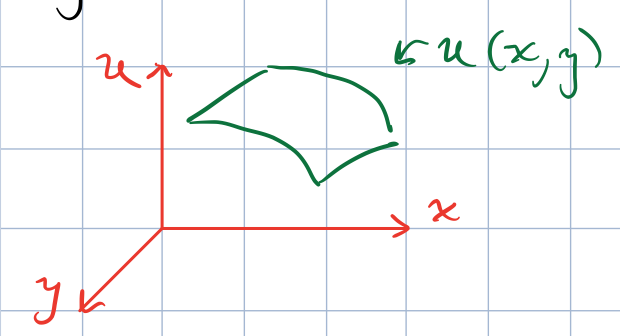
\includegraphics[scale=.75]{fig/fig1_method_characteristics.png}
	\caption{\captionStroke{Schematic integral surface.}}
	\label{fig_integral_surface}
\end{figure}

A surface $u = u(x, y)$ that solves a Cauchy problem is known as an integral
surface since integration is used to solve these problems. We can write down the
equation of this integral surface as
\begin{equation}
  F(x, y, u) \equiv u(x, y) - u = 0.
\end{equation}
Note that the first $u(x, y)$ is a function, while the second $u$ is a
variable. So for example if
\begin{equation}
  u(x, y) = x - y^2,
\end{equation}
then
\begin{equation}
  F(x, y, u) = x - y^2 - u.
\end{equation}

From vector calculus we know that any vector $\mathbf{n}$ normal to the surface $F = 0$ is given by the gradient
\begin{equation}
  \mathbf{n} = \nabla F =
  \frac{\partial u}{\partial x} \mathbf{i}
  + \frac{\partial u}{\partial y} \mathbf{j}
  - \mathbf{k}.
\end{equation}

\fref[fig_normal_vector] shows a schematic representation of this vector. The
vector is represented pointing downwards since $F = u(x, y) - u$.

\begin{figure}[h!]
	\centering 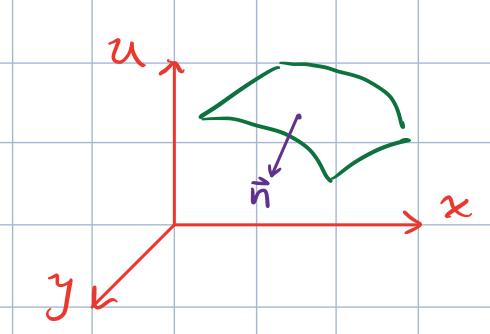
\includegraphics[scale=.75]{fig/fig2_method_characteristics.png}
	\caption{\captionStroke{Schematic integral surface with normal vector.}}
	\label{fig_normal_vector}
\end{figure}

We can rewrite the PDE as a dot product of the form
\begin{equation}
  \left\langle a(x, y), b(x, y), f(x, y, u) \right\rangle \cdot \mathbf{n} = 0.
\end{equation}

This implies that since the dot product is zero, the vector $\left\langle a(x,
y), b(x, y), f(x, y, u) \right\rangle$ must be normal to $\mathbf{n}$. Since we
stated that the vector $\mathbf{n}$ is normal to the surface $F(x, y, u) = 0$,
any vector $\mathbf{v}$ normal to $\mathbf{n}$ must lie in the tangential plane
to $F = 0$ at every point as depicted in \fref[fig_tangential_vector]
\begin{figure}[h!]
	\centering 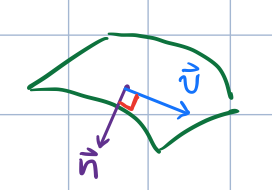
\includegraphics[scale=.75]{fig/fig3_method_characteristics.png}
	\caption{\captionStroke{Schematic integral surface with normal vector
  $\mathbf{n}$ and tangential vector $\mathbf{v}$.}}
	\label{fig_tangential_vector}
\end{figure}

But what do all these details mean? This means that the PDE requires for any
integral surface that solves the equation to be tangential to the vector
\begin{equation}
  \mathbf{v} = a(x,y) \mathbf{i} +
  b(x, y) \mathbf{j} +
  f(x, y, u) \mathbf{k}.
\end{equation}
That is, if we start at some point set by the initial condition and we move in
the direction of the vector $\mathbf{v}$ (which we can determine just by looking
at the PDE) then we move along a curve that lies entirely within the surface
$F = 0$. This curve, depicted in \fref[fig_characteristic_curve] is called a
\textit{characteristic curve}. And by finding the collection of these
characteristic curves we can therefore reconstruct the entire integral surface,
solving therefore the PDE.
\begin{figure}[h!]
	\centering \includegraphics[scale=.75]{fig/fig4_method_characteristics.png}
	\caption{\captionStroke{Schematic of a characteristic curve on an integral
  surface.}}
	\label{fig_characteristic_curve}
\end{figure}

In other words, so far we have shown that given an initial condition
$u(x, 0) = u_0(x)$ as long as we move along the direction given by the vector
$\mathbf{v} = \left\langle a(x,y), b(x,y), f(x,y,u) \right\rangle$ we are
guaranteed to lay on the integral surface. So the process to reconstruct the
entire surface would be to choose a value for $x$, then start at $u_0(x)$ and
move along $\mathbf{v}$; then we would choose a new value of $x$ and repeat the
process. At the end, the union of all these paths along the integral surface
will determine entirely the solution of the PDE. The advantage of the method as
we will show is that walking along the characteristic curve is equivalent to
solving an ODE, which for many cases we know how to do.

We can describe all the points on a characteristic curve by parametrizing
the curve with a vector function
\begin{equation}
  \mathbf{p}(t) = x(t) \mathbf{i} + y(t) \mathbf{j} + u(t) \mathbf{k}.
\end{equation}
Furthermore, we can obtain a vector tangential to this curve $\mathbf{p}(t)$ by
differentiating with respect to the parametrization variable $t$, i.e.
\begin{equation}
  \mathbf{p}'(t) = x'(t) \mathbf{i}+ y'(t) \mathbf{j} + u'(t) \mathbf{k}.
\end{equation}

Since the curve $\mathbf{p}(t)$ lays on the integral surface $F = 0$, and
$\mathbf{p}'(t)$ is tangential to this curve, that means that $\mathbf{p}'(t)$
also lies on the surface.

We stated earlier that if we move along the direction of $\mathbf{v}$ we will
reconstruct the path of the characteristic curve which we now parametrized as
$\mathbf{p}(t)$. That implies that $\mathbf{v}$ and $\mathbf{p}'(t)$ must be
pointing in the same direction, i.e.
\begin{equation}
  \mathbf{p}'(t) = \lambda \mathbf{v},
\end{equation}
where $lambda$ is a scalar. This can also be written as
\begin{equation}
  x'(t)\mathbf{i} + y'(t)\mathbf{j} + u'(t)\mathbf{k} =
  \lambda a(x,y) + \lambda b(x,y) + \lambda f(x,y,u).
\end{equation}
in other words
\begin{align}
  x'(t) = \lambda a(x,y),\\
  y'(t) = \lambda b(x,y), \\
  u'(t) = \lambda f(x,y,u).
\end{align}
We can now solve for $\lambda$ and equate all of the solutions, obtaining
\begin{equation}
  {{dx \over dt} \over a(x,y)}} =
  {{dy \over dt} \over b(x,y)} =
  {{du \over dt} \over f(x,y,u)},
\end{equation}
or simply in a compact differential form
\begin{equation}
  {dx \over a} = {dy \over b} = {du \over f}.
\end{equation}
